\documentclass{sigchi}

% Use this section to set the ACM copyright statement (e.g. for
% preprints).  Consult the conference website for the camera-ready
% copyright statement.

% Copyright
\CopyrightYear{2016}
%\setcopyright{acmcopyright}
\setcopyright{acmlicensed}
%\setcopyright{rightsretained}
%\setcopyright{usgov}
%\setcopyright{usgovmixed}
%\setcopyright{cagov}
%\setcopyright{cagovmixed}
% DOI
\doi{http://dx.doi.org/10.475/123_4}
% ISBN
\isbn{123-4567-24-567/08/06}
%Conference
\conferenceinfo{CHI'16,}{May 07--12, 2016, San Jose, CA, USA}
%Price
\acmPrice{\$15.00}

% Use this command to override the default ACM copyright statement
% (e.g. for preprints).  Consult the conference website for the
% camera-ready copyright statement.


%% HOW TO OVERRIDE THE DEFAULT COPYRIGHT STRIP --
%% Please note you need to make sure the copy for your specific
%% license is used here!
% \toappear{
% Permission to make digital or hard copies of all or part of this work
% for personal or classroom use is granted without fee provided that
% copies are not made or distributed for profit or commercial advantage
% and that copies bear this notice and the full citation on the first
% page. Copyrights for components of this work owned by others than ACM
% must be honored. Abstracting with credit is permitted. To copy
% otherwise, or republish, to post on servers or to redistribute to
% lists, requires prior specific permission and/or a fee. Request
% permissions from \href{mailto:Permissions@acm.org}{Permissions@acm.org}. \\
% \emph{CHI '16},  May 07--12, 2016, San Jose, CA, USA \\
% ACM xxx-x-xxxx-xxxx-x/xx/xx\ldots \$15.00 \\
% DOI: \url{http://dx.doi.org/xx.xxxx/xxxxxxx.xxxxxxx}
% }

% Arabic page numbers for submission.  Remove this line to eliminate
% page numbers for the camera ready copy
% \pagenumbering{arabic}

% Load basic packages
\usepackage{balance}       % to better equalize the last page
\usepackage{graphics}      % for EPS, load graphicx instead 
\usepackage[T1]{fontenc}   % for umlauts and other diaeresis
\usepackage{txfonts}
\usepackage{mathptmx}
\usepackage[pdflang={en-US},pdftex]{hyperref}
\usepackage{color}
\usepackage{booktabs}
\usepackage{textcomp}

% Some optional stuff you might like/need.
\usepackage{microtype}        % Improved Tracking and Kerning
% \usepackage[all]{hypcap}    % Fixes bug in hyperref caption linking
\usepackage{ccicons}          % Cite your images correctly!
% \usepackage[utf8]{inputenc} % for a UTF8 editor only
\usepackage{float}

% If you want to use todo notes, marginpars etc. during creation of
% your draft document, you have to enable the "chi_draft" option for
% the document class. To do this, change the very first line to:
% "\documentclass[chi_draft]{sigchi}". You can then place todo notes
% by using the "\todo{...}"  command. Make sure to disable the draft
% option again before submitting your final document.
\usepackage{todonotes}

% Paper metadata (use plain text, for PDF inclusion and later
% re-using, if desired).  Use \emtpyauthor when submitting for review
% so you remain anonymous.
\def\plaintitle{}
\def\plainauthor{First Author, Second Author, Third Author,
  Fourth Author, Fifth Author, Sixth Author}
\def\emptyauthor{}
\def\plainkeywords{Authors' choice; of terms; separated; by
  semicolons; include commas, within terms only; required.}
\def\plaingeneralterms{Documentation, Standardization}

% llt: Define a global style for URLs, rather that the default one
\makeatletter
\def\url@leostyle{%
  \@ifundefined{selectfont}{
    \def\UrlFont{\sf}
  }{
    \def\UrlFont{\small\bf\ttfamily}
  }}
\makeatother
\urlstyle{leo}

% To make various LaTeX processors do the right thing with page size.
\def\pprw{8.5in}
\def\pprh{11in}
\special{papersize=\pprw,\pprh}
\setlength{\paperwidth}{\pprw}
\setlength{\paperheight}{\pprh}
\setlength{\pdfpagewidth}{\pprw}
\setlength{\pdfpageheight}{\pprh}

% Make sure hyperref comes last of your loaded packages, to give it a
% fighting chance of not being over-written, since its job is to
% redefine many LaTeX commands.
\definecolor{linkColor}{RGB}{6,125,233}
\hypersetup{%
  pdftitle={\plaintitle},
% Use \plainauthor for final version.
%  pdfauthor={\plainauthor},
  pdfauthor={\emptyauthor},
  pdfkeywords={\plainkeywords},
  pdfdisplaydoctitle=true, % For Accessibility
  bookmarksnumbered,
  pdfstartview={FitH},
  colorlinks,
  citecolor=black,
  filecolor=black,
  linkcolor=black,
  urlcolor=linkColor,
  breaklinks=true,
  hypertexnames=false
}

% create a shortcut to typeset table headings
% \newcommand\tabhead[1]{\small\textbf{#1}}

% End of preamble. Here it comes the document.
\begin{document}

\title{Milestone 2\\ Discovering Unaligned Expectations in Universities and Industry for New Graduates in Computer Science and Software Engineering and Finding Possible Solutions}

\numberofauthors{2}
\author{%
  \alignauthor{Alan Franzoni\\
    \affaddr{Georgia Institute of Technology}\\
    \affaddr{Trieste, Italy}\\
    \email{alan.franzoni@gatech.edu}}\\
  \alignauthor{Hasti Ghabel\\
    \affaddr{Georgia Institute of Technology}\\
    \affaddr{Atlanta, GA}\\
    \email{hghabel1@gatech.edu}}\\
}

\maketitle

\section{About our research}
We focus on discovering whether there is a misalignment in university and industry expectations for new graduates. We are considering four groups including: 1-undergraduate students, 2-post-graduate students,3- professors, teachers, or university staff, and 4-industry professionals. We are also collecting the data on what would be some possible solutions to reduce the skill gap, which is caused by expectation gap among these four groups.

\textit{\textbf{Our Research Questions}}\newline
We will direct two sets of questions in our final project. In the first set, our main question is: \textbf{does the perceived skill gap in fresh graduates exist because the academy is unable to provide a good training, or just because a) the academy is not even trying to do that kind of job, and b) the industry is taking that kind of job for granted, or c) the students think they should be getting something that the university has no intention to provide them with?} Here, we ask what could be the reasons that there exist a gap between students, professors, and industry professionals' expectations. We will look into these questions for both \textbf{undergraduate} and \textbf{post-graduate} level students that are recently graduated from school. We also ask the question that \textbf{how the students' degree can improve the chance of getting hired? Do the graduate-level studies help the students to gain adaptive skills in industry more quickly?}\newline
In the second set of our questions, we are asking \textbf{what would be the best solutions that bring the university and industry's objectives closer to each other?} 
latexmk -pdf Milestone2.tex

\textit{\textbf{Our Hypothesis}}\newline
\textit{Hypothesis 1}: One of the reasons for the perceived skill gap is that all those that should - in an employer's view - care for learning some skills to be used at work, don't actually have that aim during their education phase. In other words, the misaligned expectations between industry and university causes the skill gap. Those skills have impact on job proficiency and possibilities to get hired. We think that the expectations among four groups differ. These four groups are composed of \textbf{undergraduate-level students, post-graduate-level students, educators and school staff, and industry professionals}. The main problem is not only that one side hasn’t enough resources or skills to achieve a certain goal, but, rather, that there’s a different vision or gaol on what should be done, and different and unaligned \textit{rewards} exist for different groups.  

\textit{Hypothesis 2}:  We think that the following hypothesis is that the graduate-level studies, on the contrary, can play an important role on reducing the skill gap between industry and university, and therefore, can be considered as one good resolution for that issue. More specifically, we think that \textbf{high-quality online graduate-level programs} such as Georgia Tech OMSCS (Online Master of Science in Computer Science) are quite aligned with industry expectations. These such programs also target many people from all over the world, who can become proficient in their job quickly as well as being active in an academic environment.

\section{review research methodologies}
During this milestone, we collected data for four categories: "undergraduate students", "post-graduate students", "professors, teachers, and assistants", and "industry professionals".
We provided one single survey for all participants. We added one question of multiple choice describing each category. Each survey taker had the option of selecting one or multiple categories that best describe their current position. The link of our survey is as below:\\

\textbf{Survey link}: \url{https://goo.gl/forms/Lf2OrO57QuI5nUe32}\\

We provided a website, where we describe the goals of the research, explain a short description about ourselves, give access to our survey, and display other informations. In order to recruit many participants, we shared our website with different groups and asked them to take our survey. The participants or whoever interested is able to subscribe to our website and receive the results. You can find our website under this link \url{http://www.misalignedtech.com/}\\
Recruiting survey takers from different categories was a big challenge for us. The biggest challenge was to recruit enough undergraduate students and professors, teachers and assistants. We think that summer time is one of the reasons that we could not recruit enough undergraduate students, since most of students do not take courses during summer. Similarly, teachers and professors might be off during summer time or they might be more focused on their research topics. Some of the methods we used to share our survey with the people in different categories are as below:
\begin{itemize}
	\item Shared our website link via Piazza with our classmates
	\item Provided our survey in Peer-Survey platform: \url{http://peersurvey.cc.gatech.edu/}
	\item Shared our website link in OMSCS Google Plus platform
	\item Per confirmation, sent an email including our website link to the tech team of our company
	\item Shared the survey with EESTech Student Association in Europe (a student organization)
	\item Sent the email to some of the professors at Georgia Tech and Georgia State University
\end{itemize}

Another challenge during this milestone was to learn R programming and apply it on our analysis. We faced many syntax or programming errors, which took a lot of time to resolve them and make sure the data is in the right format and we can provide the correct graphs.

\section{Results}
We were able to collect the total of 119 responses from all four categories. The break down for each category is as: Undergraduate Students = 4 responses, Graduate Students = 52, Professor, Teachers, and Assistants = 2 responses, and Industry Professionals = 46 responses.
We will go through the results in the following sections.

\textit{\textbf{General Information}}\newline
The age of most of the participants in this category was in the range of 26 to 35 year old (53.8\%). The next two big age range were 36-45 and 18-25 years old with percentage of 16.8\% and 15.1\%, respectively (figure 1). The latest earned degree of participants were as follow: 62.2\% earned Bachelor's degree, 24.4\% have Master's degree, 6.7\% have Doctorate degree, and 5.9\% have already High School diploma.

\begin{figure}
\centering
  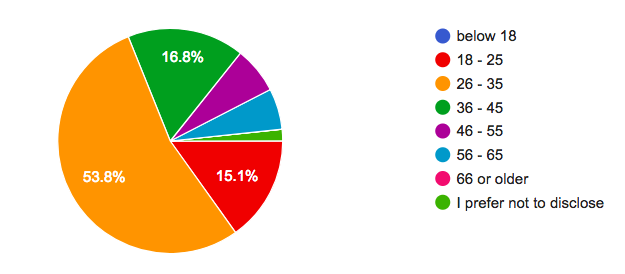
\includegraphics[width=1.05\columnwidth]{figures/age_range}
  \caption{The break down of the age range of the participants}~\label{fig:figure 1}
\end{figure}

\textit{\textbf{Essential Factors to Get Hired}}\newline
We looked at some factors such as GPA that might play a role in finding a job for new graduates. We compared the effect of GPA for undergraduate and post-graduate students on landing their first job after graduation. Most of the responses show that high GPA is not essential, but low GPA can discourage the employer for hiring the candidate. Interestingly, this option has the highest selected value for both categories. 61\% of responses relates to undergraduate students and 48\% relates to graduate students. One interesting point is that 18\% of the responses point out that high undergraduate GPA is not essential at all in landing the first job. However, 42\% of responses say that high post-graduate GPA is not relevant at all in getting hired for the first time (figure 2). 

\begin{figure}
\centering
  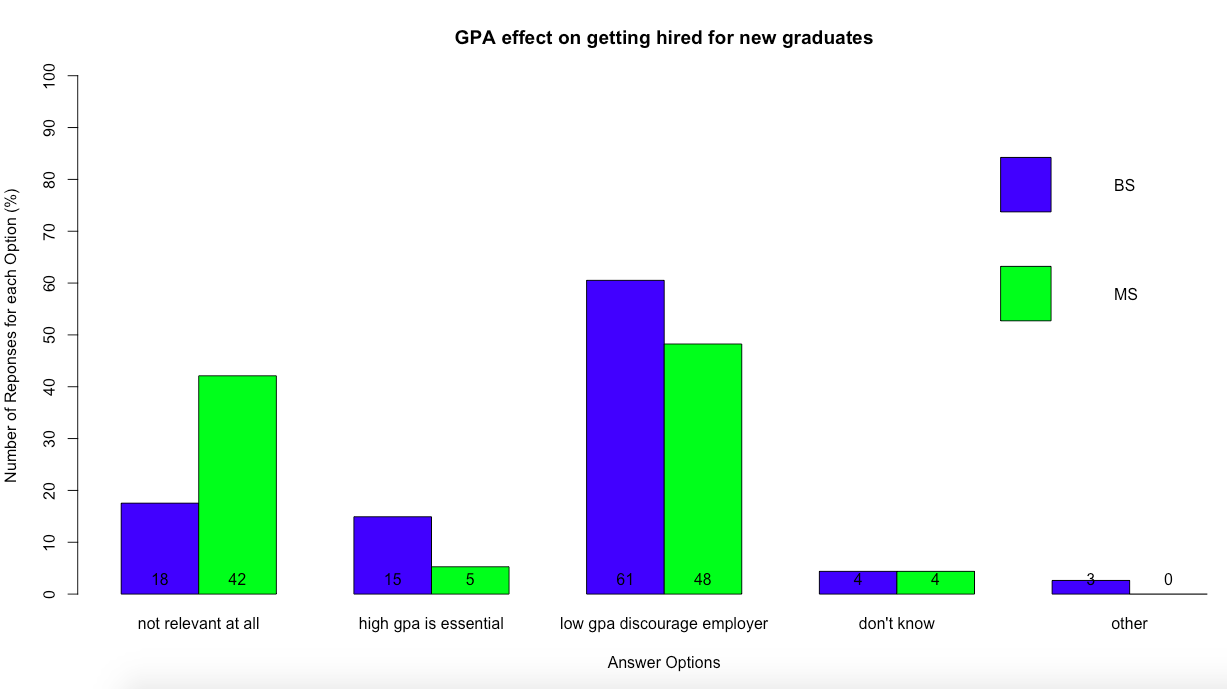
\includegraphics[width=1.05\columnwidth]{figures/gpa_effect_on_hiring_BS_MS}
  \caption{Display the effect of GPA on landing the first job for undergraduate and graduate students. The blue bars show the results for number of responses for new graduates in undergraduate level and the green bars are related to graduate level. The x-axis shows the answer options and the y-axis is the percentage of the selected option.}~\label{fig:figure 2}
\end{figure}

In the next step, we looked at the time period for new graduates to get hired, in both undergraduate and post-graduate levels. As we see in figure 3, around 37\% of the responses describe that a new graduate in post-graduate level has already a job, comparing to 20\% of the same response for undergraduate-level graduates. One of the results we can explain from the responses is that the graduate-level studies can better prepare students for job industry. Therefore, they have higher percentage of having a job during their studies.

\begin{figure}
\centering
  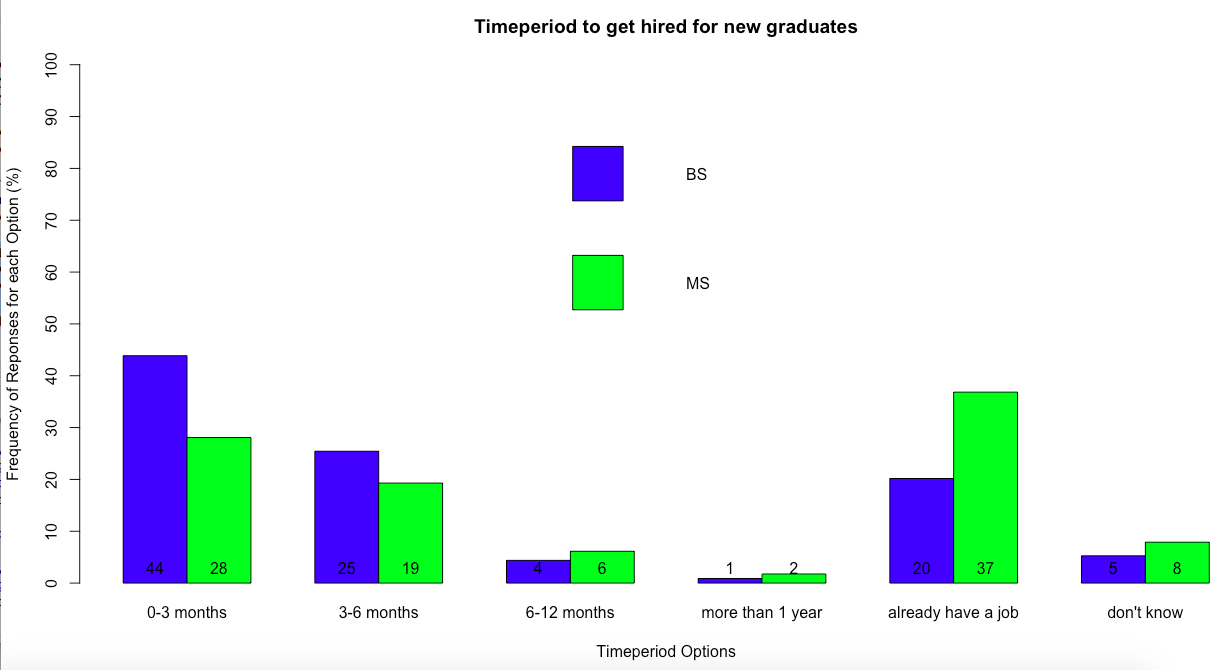
\includegraphics[width=1.05\columnwidth]{figures/timeperiod_to_get_hired_BS_MS}
  \caption{Display the time period of getting hired for new graduates in undergraduate and post-graduate levels. The blue bars show the results for number of responses for new graduates in undergraduate level and the green bars are related to graduate level. The x-axis shows the answer options and the y-axis is the percentage of the selected option.}~\label{fig:figure 3}
\end{figure}

\textit{\textbf{Essential Factors to Become Proficient in Job}}\newline
We also looked at the job proficiency and compared it between new graduates from undergraduate and post-graduate levels. We collect the data regarding the time period for these two groups to become proficient in their job right after they get hired. Among available time ranges, the peak of time period for both groups exists at 6-12 months (figure 4). When we compare BS and MS graduates, it shows that higher percentages were selected for MS graduates at those shorter time periods. In other words, 14\% of participants think that MS graduates become fully proficient in their job after 0-3 months, where only 4\% select this time period for BS graduates. Similarly, 29\% of participants think that MS graduates need 3-6 months to become fully proficient and on the other hand only 12\% voted this option for BS graduates. We can see that longer time periods relate to the BS graduates including 12-24 months and more than 2 years (figure 4).

\begin{figure}
\centering
  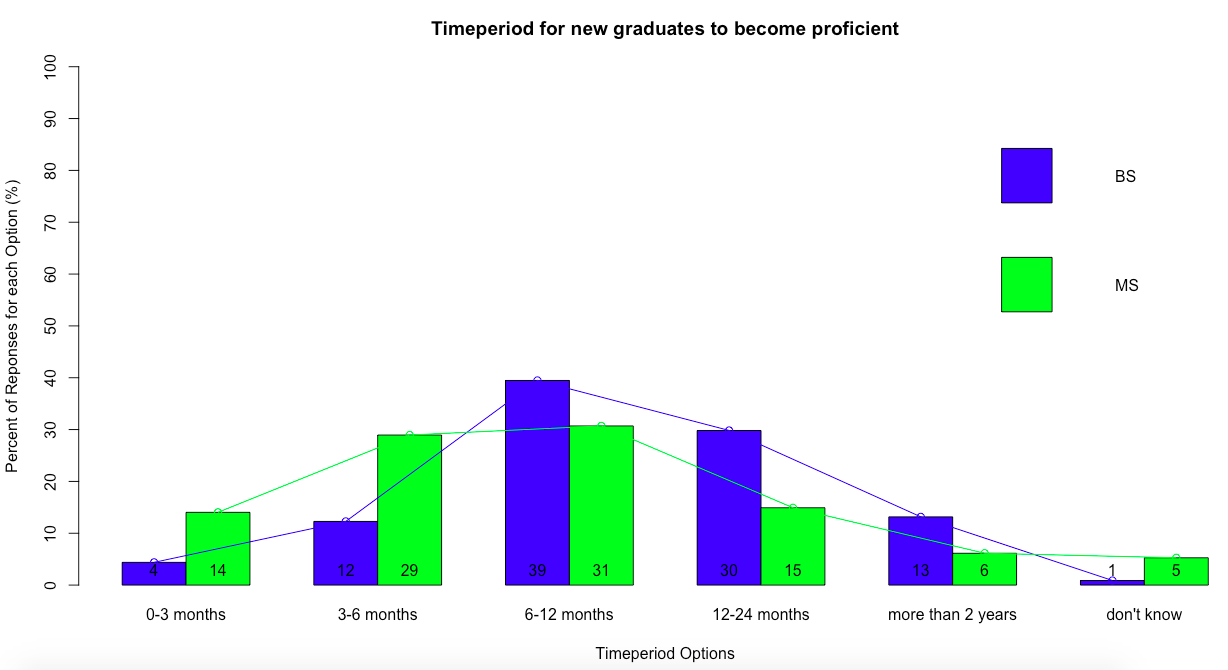
\includegraphics[width=1.05\columnwidth]{figures/timeperiod_proficiency_BS_MS_with_trendline}
  \caption{Display the time period of becoming fully proficient in their jobs after new graduates in undergraduate and post-graduate levels get hired. The blue bars show the results for number of responses for new graduates in undergraduate level and the green bars are related to graduate level. The x-axis shows the answer options and the y-axis is the percentage of the selected option.}~\label{fig:figure 4}
\end{figure}

\textit{\textbf{Compare New BS and MS Graduates Vs. an Experienced Candidate}}\newline
We were interested to see whether degree or experience can be recognized as an essential factor of getting a job and becoming proficient in it. For this reason, we provided  three scenarios to compare the fresh graduates with experienced candidates.\\
The first scenario asks about the chances of getting hired for two groups. The first group compares a fresh BS graduate with a candidate without a degree, but having 4 years of experience in the same or similar position. The second group is the comparison between the fresh MS graduate and a candidate with BS degree and 2 years of relative work experience. Based on the responses, the chances for both fresh graduates are the same (22\%) and the experienced candidates have higher chances (53\%) of getting hired compared to fresh BS or MS graduates. Around 18\% of the responses selected the option that the chances for a fresh graduate and experienced candidate are the same. The results show in figure 5.

\begin{figure}
\centering
  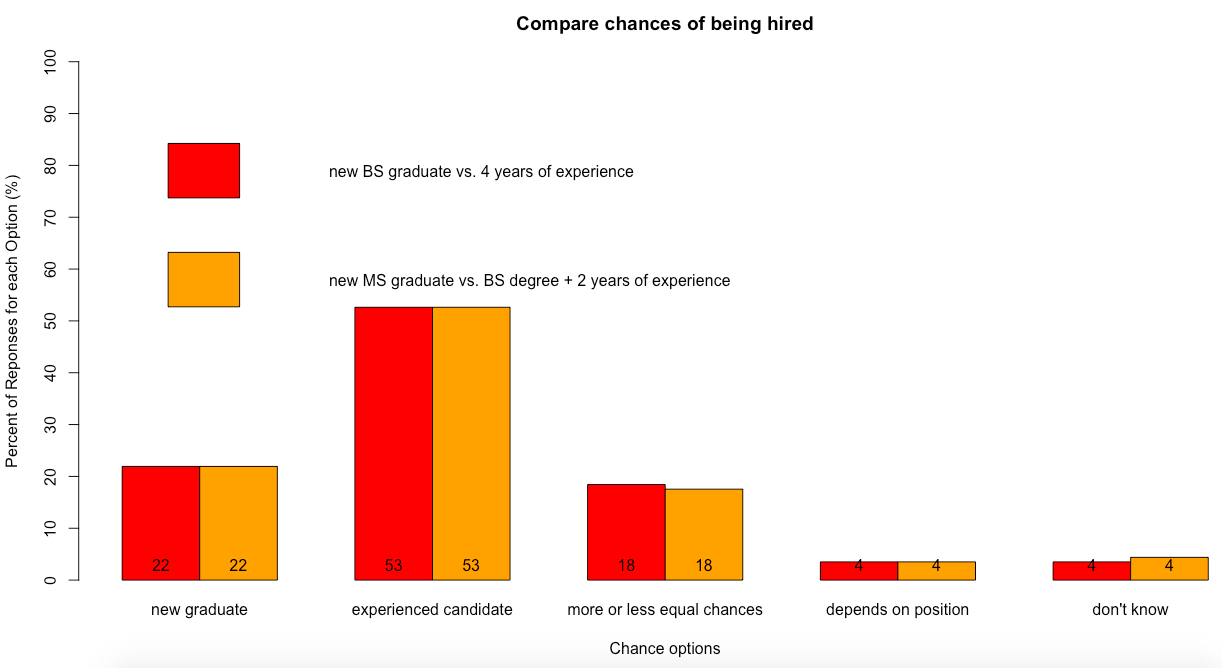
\includegraphics[width=1.05\columnwidth]{figures/compare_BS_MS_exp_job_chances}
  \caption{Display comparison of chances of getting hired for new graduates and an experienced candidate. The red bars show the result for the category of comparing a fresh BS graduate with a 4 years of experienced candidate with no degree. The orange bars compare the fresh MS graduate with a candidate, who has a BS degree with 2 years of experience. The x-axis shows the options or categories, who have higher percentage of getting hired.}~\label{fig:figure 5}
\end{figure}

We provided the same scenario described above to compare the two groups' proficiency right after and after 1 year of getting hired. The results shows in figure 6 and 7.

\begin{figure}
\centering
  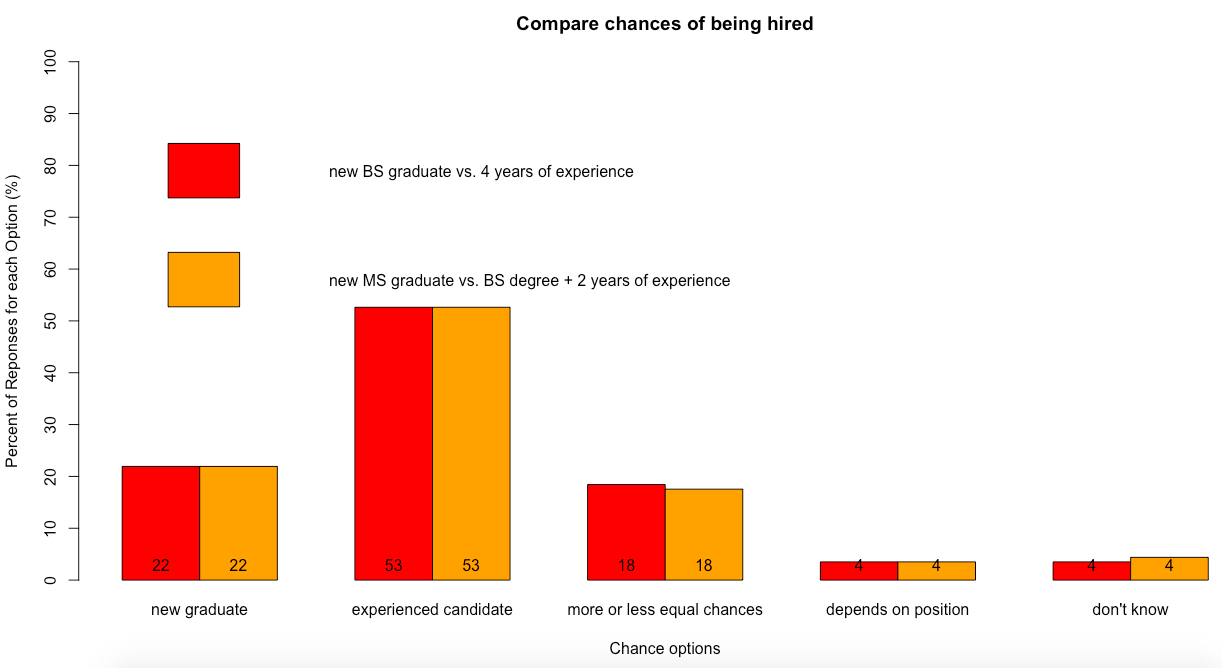
\includegraphics[width=1.05\columnwidth]{figures/compare_BS_MS_exp_job_chances}
  \caption{Display comparison of chances of getting hired for new graduates and an experienced candidate. The red bars show the result for the category of comparing a fresh BS graduate with a 4 years of experienced candidate with no degree. The orange bars compare the fresh MS graduate with a candidate, who has a BS degree with 2 years of experience. The x-axis shows the options or categories, who have higher percentage of getting hired.}~\label{fig:figure 6}
\end{figure}

\begin{figure}
\centering
  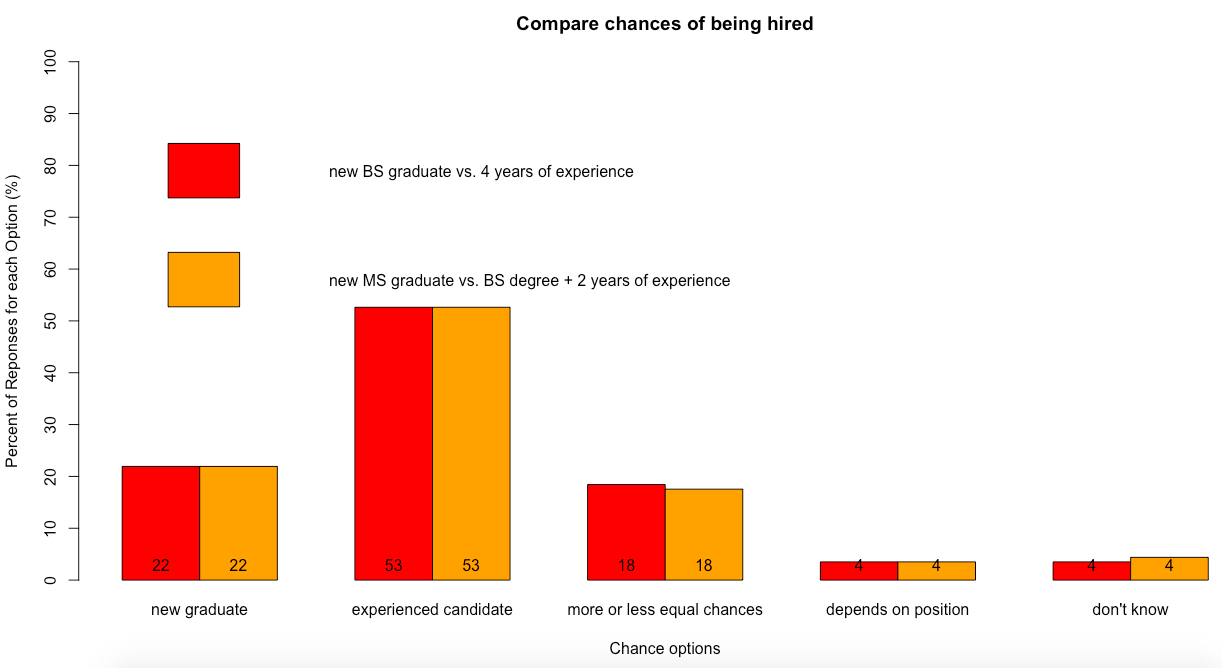
\includegraphics[width=1.05\columnwidth]{figures/compare_BS_MS_exp_job_chances}
  \caption{Display comparison of chances of getting hired for new graduates and an experienced candidate. The red bars show the result for the category of comparing a fresh BS graduate with a 4 years of experienced candidate with no degree. The orange bars compare the fresh MS graduate with a candidate, who has a BS degree with 2 years of experience. The x-axis shows the options or categories, who have higher percentage of getting hired.}~\label{fig:figure 7}
\end{figure}

\textit{\textbf{Undergraduate and Graduate Level Expectations and Goals}}\newline

We're still collecting and analyzing data; we're using R in order to pick up the data, and try to determine whether there's a correlation.\newline
An example of our analysis script and data can be found here:

\href{https://www.dropbox.com/s/hs6p85pte1o8tie/answers_pare.R?dl=0}{R analysis script}

\href{https://www.dropbox.com/s/mbvigipou0txxeh/answers2.csv?dl=0}{Survey sample data}

So far (but the analysis is still undergoing, we had to refresh our statistic knowledge quite a lot, and our R knowledge was non-existent - we managed to properly normalize data for analysis and started doing some linear regression, so far), we haven't found a tremendous amount of correlation between variables, even though some expected results seem to exist: as an example, there're more industry professionals thinking that a BSc doesn't mean to learn programming, compared to non-professionals.


\textit{\textbf{Ideas for Possible Solutions}}\newline
We asked participants to share their thoughts on how can students gain work experience during their undergraduate or post-graduate studies. Most of the suggestions were similar among both categories. We summarized some of the suggested options below:
\begin{itemize}
	\item Internships
	\item Open-source projects and part-time job experiences
	\item Work on real-world problems with an industry partner
	\item Research on interesting projects
	\item Volunteering on side-projects
\end{itemize}

We asked the question of alternatives to Master's degree for a professional in need of training.  The options were multi-selected and the top three selected items and some other responses are as below:
\begin{enumerate}
	\item Massive Open Online Courses (MOOC) (67\%)
	\item Retraining in Job professional (64\%)
	\item In-person and non-academic institutions (38\%)
	\item Bootcamps (\~ 1\%)
	\item Better undergraduate study and learning (\~ 1\%)
\end{enumerate}

According to the previous question, we investigated the benefits of joining an online graduate-level program. We can mention some of the benefits as below.
\begin{itemize}
	\item Time and schedule flexibility (84\%).
	\item Lower tuitions (68\%).
	\item Motivation and interest on the topic not just an imposed training experience (55\%).
	\item Career advancement to guarantee for a better position (52\%).
\end{itemize}

In the end, we asked the participants which of the following sentences are more accurate:\\

1- The BS students are already prepared to join the industry and they do not need a higher post-graduate degree.\\
2- The MS students are more prepared than undergraduate-level students.\\
3- Regardless of academic degree, anybody entering the workforce for the first time will need training and time to get fully proficient.\\

Surprisingly, about 76\% of participants agree on option 3. Following that, about 19\% selected option 2 and only 5\% selected option 1. This shows that the experience gives better skills and preparation to join industry. This can describe the gap between expectations and goals of academic and industry. We also can see that post-graduate studies better prepare students for joining industry and therefore, we can say that the goals of post-graduate level studies are closer to industry.

\begin{figure}
\centering
  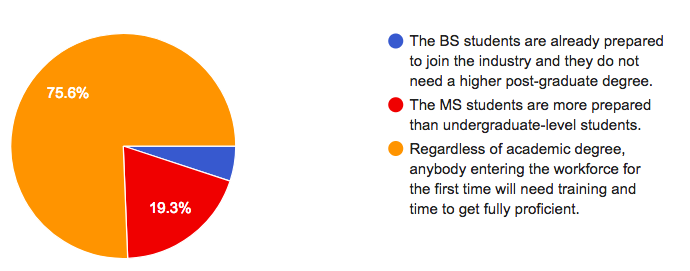
\includegraphics[width=1.05\columnwidth]{figures/general_accurate_sentence}
  \caption{Display comparison of general idea of participants.}~\label{fig:figure 8}
\end{figure}

\section{Progress Report}
During this milestone, we were able to create the final draft of our survey and share it with many different groups, which fit our categories. We were able to collect total of 119 responses. However, we faced a big challenge of recruiting undergraduate students and professors, teachers or assistants categories.

Some of our achievements were setting up R programming IDE and improve our knowledge in this language. We analyzed the data and plotted many graphs with R. However, we faced many challenges on debugging and resolving the errors.

 \section{Future Steps}
In our next step, we are planning to collect all the responses and complete our survey data. We keep the survey open till July 20th and then we would not receive any further responses. We will continue our analysis on the data when we have all the responses completed.

We will start working on final project and providing graphs for the final paper. When the project is completed, we will share our results on our website for whoever is interested to see the results.

 

\balance{}

\balance{}

% REFERENCES FORMAT
% References must be the same font size as other body text.
%\bibliographystyle{SIGCHI-Reference-Format}
%\bibliography{../bibliography.bib}

\end{document}

%%% Local Variables:
%%% mode: latex
%%% TeX-master: t
%%% End:
 